%% Creator: Inkscape inkscape 0.92.2, www.inkscape.org
%% PDF/EPS/PS + LaTeX output extension by Johan Engelen, 2010
%% Accompanies image file 'fle3.eps' (pdf, eps, ps)
%%
%% To include the image in your LaTeX document, write
%%   \input{<filename>.pdf_tex}
%%  instead of
%%   \includegraphics{<filename>.pdf}
%% To scale the image, write
%%   \def\svgwidth{<desired width>}
%%   \input{<filename>.pdf_tex}
%%  instead of
%%   \includegraphics[width=<desired width>]{<filename>.pdf}
%%
%% Images with a different path to the parent latex file can
%% be accessed with the `import' package (which may need to be
%% installed) using
%%   \usepackage{import}
%% in the preamble, and then including the image with
%%   \import{<path to file>}{<filename>.pdf_tex}
%% Alternatively, one can specify
%%   \graphicspath{{<path to file>/}}
%% 
%% For more information, please see info/svg-inkscape on CTAN:
%%   http://tug.ctan.org/tex-archive/info/svg-inkscape
%%
\begingroup%
  \makeatletter%
  \providecommand\color[2][]{%
    \errmessage{(Inkscape) Color is used for the text in Inkscape, but the package 'color.sty' is not loaded}%
    \renewcommand\color[2][]{}%
  }%
  \providecommand\transparent[1]{%
    \errmessage{(Inkscape) Transparency is used (non-zero) for the text in Inkscape, but the package 'transparent.sty' is not loaded}%
    \renewcommand\transparent[1]{}%
  }%
  \providecommand\rotatebox[2]{#2}%
  \ifx\svgwidth\undefined%
    \setlength{\unitlength}{575.9999856bp}%
    \ifx\svgscale\undefined%
      \relax%
    \else%
      \setlength{\unitlength}{\unitlength * \real{\svgscale}}%
    \fi%
  \else%
    \setlength{\unitlength}{\svgwidth}%
  \fi%
  \global\let\svgwidth\undefined%
  \global\let\svgscale\undefined%
  \makeatother%
  \begin{picture}(1,0.66111111)%
    \put(0,0){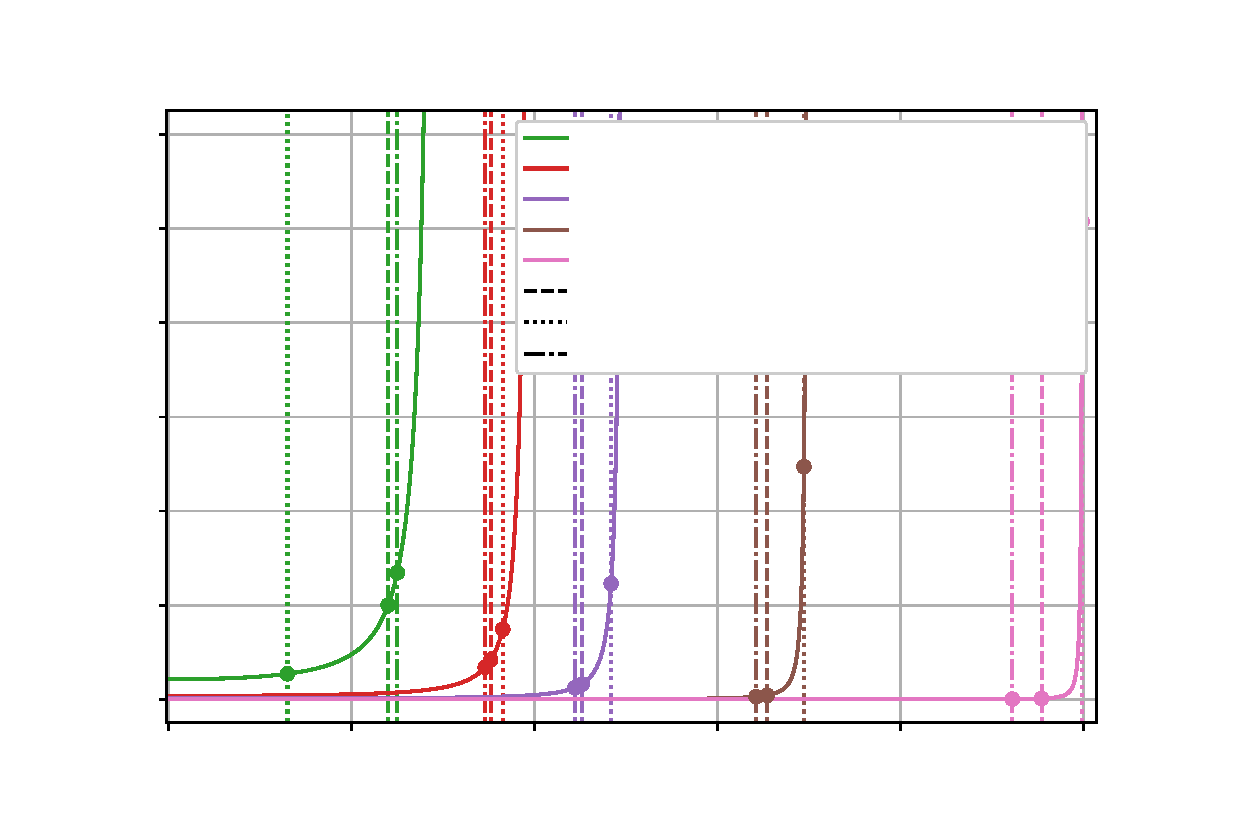
\includegraphics[width=\unitlength]{images_2ddl/fle3.eps}}%
    \put(0.12102726,0.04753889){\color[rgb]{0,0,0}\makebox(0,0)[lb]{\smash{0}}}%
    \put(0.26804688,0.04753889){\color[rgb]{0,0,0}\makebox(0,0)[lb]{\smash{10}}}%
    \put(0.42058854,0.04753889){\color[rgb]{0,0,0}\makebox(0,0)[lb]{\smash{20}}}%
    \put(0.57312847,0.04753889){\color[rgb]{0,0,0}\makebox(0,0)[lb]{\smash{30}}}%
    \put(0.7256684,0.04753889){\color[rgb]{0,0,0}\makebox(0,0)[lb]{\smash{40}}}%
    \put(0.87821007,0.04753889){\color[rgb]{0,0,0}\makebox(0,0)[lb]{\smash{50}}}%
    \put(0.1018066,0.08574358){\color[rgb]{0,0,0}\makebox(0,0)[lb]{\smash{0}}}%
    \put(0.1018066,0.16424358){\color[rgb]{0,0,0}\makebox(0,0)[lb]{\smash{2}}}%
    \put(0.1018066,0.24274306){\color[rgb]{0,0,0}\makebox(0,0)[lb]{\smash{4}}}%
    \put(0.1018066,0.32124306){\color[rgb]{0,0,0}\makebox(0,0)[lb]{\smash{6}}}%
    \put(0.1018066,0.39974306){\color[rgb]{0,0,0}\makebox(0,0)[lb]{\smash{8}}}%
    \put(0.09076615,0.47824306){\color[rgb]{0,0,0}\makebox(0,0)[lb]{\smash{10}}}%
    \put(0.09076615,0.55674132){\color[rgb]{0,0,0}\makebox(0,0)[lb]{\smash{12}}}%
    \put(0.07972552,0.28014063){\color[rgb]{0,0,0}\rotatebox{90}{\makebox(0,0)[lb]{\smash{$H_{max} (m)$}}}}%
    \put(0.47221181,0.55419097){\color[rgb]{0,0,0}\makebox(0,0)[lb]{\smash{$r_2=15 mm$}}}%
    \put(0.47221181,0.52872049){\color[rgb]{0,0,0}\makebox(0,0)[lb]{\smash{$r_2=20 mm$}}}%
    \put(0.47221181,0.50324826){\color[rgb]{0,0,0}\makebox(0,0)[lb]{\smash{$r_2=25 mm$}}}%
    \put(0.47221181,0.47777604){\color[rgb]{0,0,0}\makebox(0,0)[lb]{\smash{$r_2=35 mm$}}}%
    \put(0.47221181,0.45230382){\color[rgb]{0,0,0}\makebox(0,0)[lb]{\smash{$r_2=50 mm$}}}%
    \put(0.47221181,0.4268316){\color[rgb]{0,0,0}\makebox(0,0)[lb]{\smash{limite en flambement/écoulement}}}%
    \put(0.47221181,0.40065451){\color[rgb]{0,0,0}\makebox(0,0)[lb]{\smash{$\delta / R>0.1$}}}%
    \put(0.47221181,0.37447743){\color[rgb]{0,0,0}\makebox(0,0)[lb]{\smash{limite en écoulement saut pieds joints}}}%
    \put(0.475,0.02){\color[rgb]{0,0,0}\makebox(0,0)[lb]{\smash{$r_1(mm)$}}}%
  \end{picture}%
\endgroup%
